\documentclass{ecnreport}

\stud{OD Robotique}
\topic{Aerial and underwater robots}

\begin{document}

\inserttitle{Aerial and underwater robots}

\insertsubtitle{AUV simulation and control}

\section{Content of this lab}

The goal of this lab is to design a thruster-propelled Autonomous Underwater Vehicle (AUV). After the geometric design, a rough approximation of the hydrodynamic damping will be computed
and low-level control (PID's) will be tuned. At the end, the AUV should be able to follow a trajectory defined with a sequence of waypoints.

\subsection{Installing the simulator}

The simulator is in a ROS package called \texttt{freefloating\_gazebo} and should be already installed on the P-ro computers.\\
The actual package that you will modify is downloaded (in \texttt{\~{}/ros/src}) with \texttt{rosdl ecn\_rasom}\footnote{to use your own computer, git should be used to clone https://github.com/oKermorgant/ecn\_rasom.git}

This package has the classical ROS structure:
\begin{figure}[h]
\begin{minipage}{.25\linewidth} ~ \end{minipage}
\begin{minipage}{.5\linewidth}
 \dirtree{%
.1 ecn\_rasom. 
.2 config.
.3 waypoints.yaml.
.2 launch.
.3 auv.launch.
.3 auv\_estim.launch.
.3 ekf.launch.
.2 scripts.
.2 src.
.3 waypoint.cpp.
.2 subject.
.2 urdf.
.3 auv.xacro.
.2 package.xml.
.2 CMakeLists.txt.
} 
\end{minipage}
%\begin{minipage}{.2\linewidth} ~ \end{minipage}
\caption{Files used by the simulator}
\end{figure}

%\subsection{First run of Gazebo}
%
%It was noticed on some computers that the first launch of Gazebo can take some time. In order to check, launch this empty world simulation:
%\begin{center}\defaultstyle
%\begin{lstlisting}
%roslaunch gazebo_ros empty_world.launch
%  \end{lstlisting}
%  \end{center}
%  When the Gazebo GUI is displayed, type\texttt{Ctrl-C} in order to end the programs.

\section{Waypoint following}

The first task is to finish the waypoint following node defined in \texttt{waypoint.cpp}. This node already loads the waypoints defined in \texttt{waypoints.yaml} but does not follow them yet.
These waypoints should be modified according to the trajectory you want the robot to follow. A waypoint is defined by its $(x,y,z,\theta)$ values where $\theta$ is the yaw angle. Look at the current
code to see how to change a yaw angle to a quaternion needed by the \texttt{PoseStamped} message.\\

Topics can be renamed or the node can be run through a launch file in order to be in the \texttt{/auv} namespace.
The simulation can then be run with:
\begin{itemize}
 \item \texttt{roslaunch ecn\_rasom auv.launch} for all built-in nodes
 \item \texttt{rosrun ecn\_rasom waypoint} for yours
\end{itemize}
which leads to the following graph where \texttt{/auv/wp} is your node.
\begin{figure}[h]\centering
 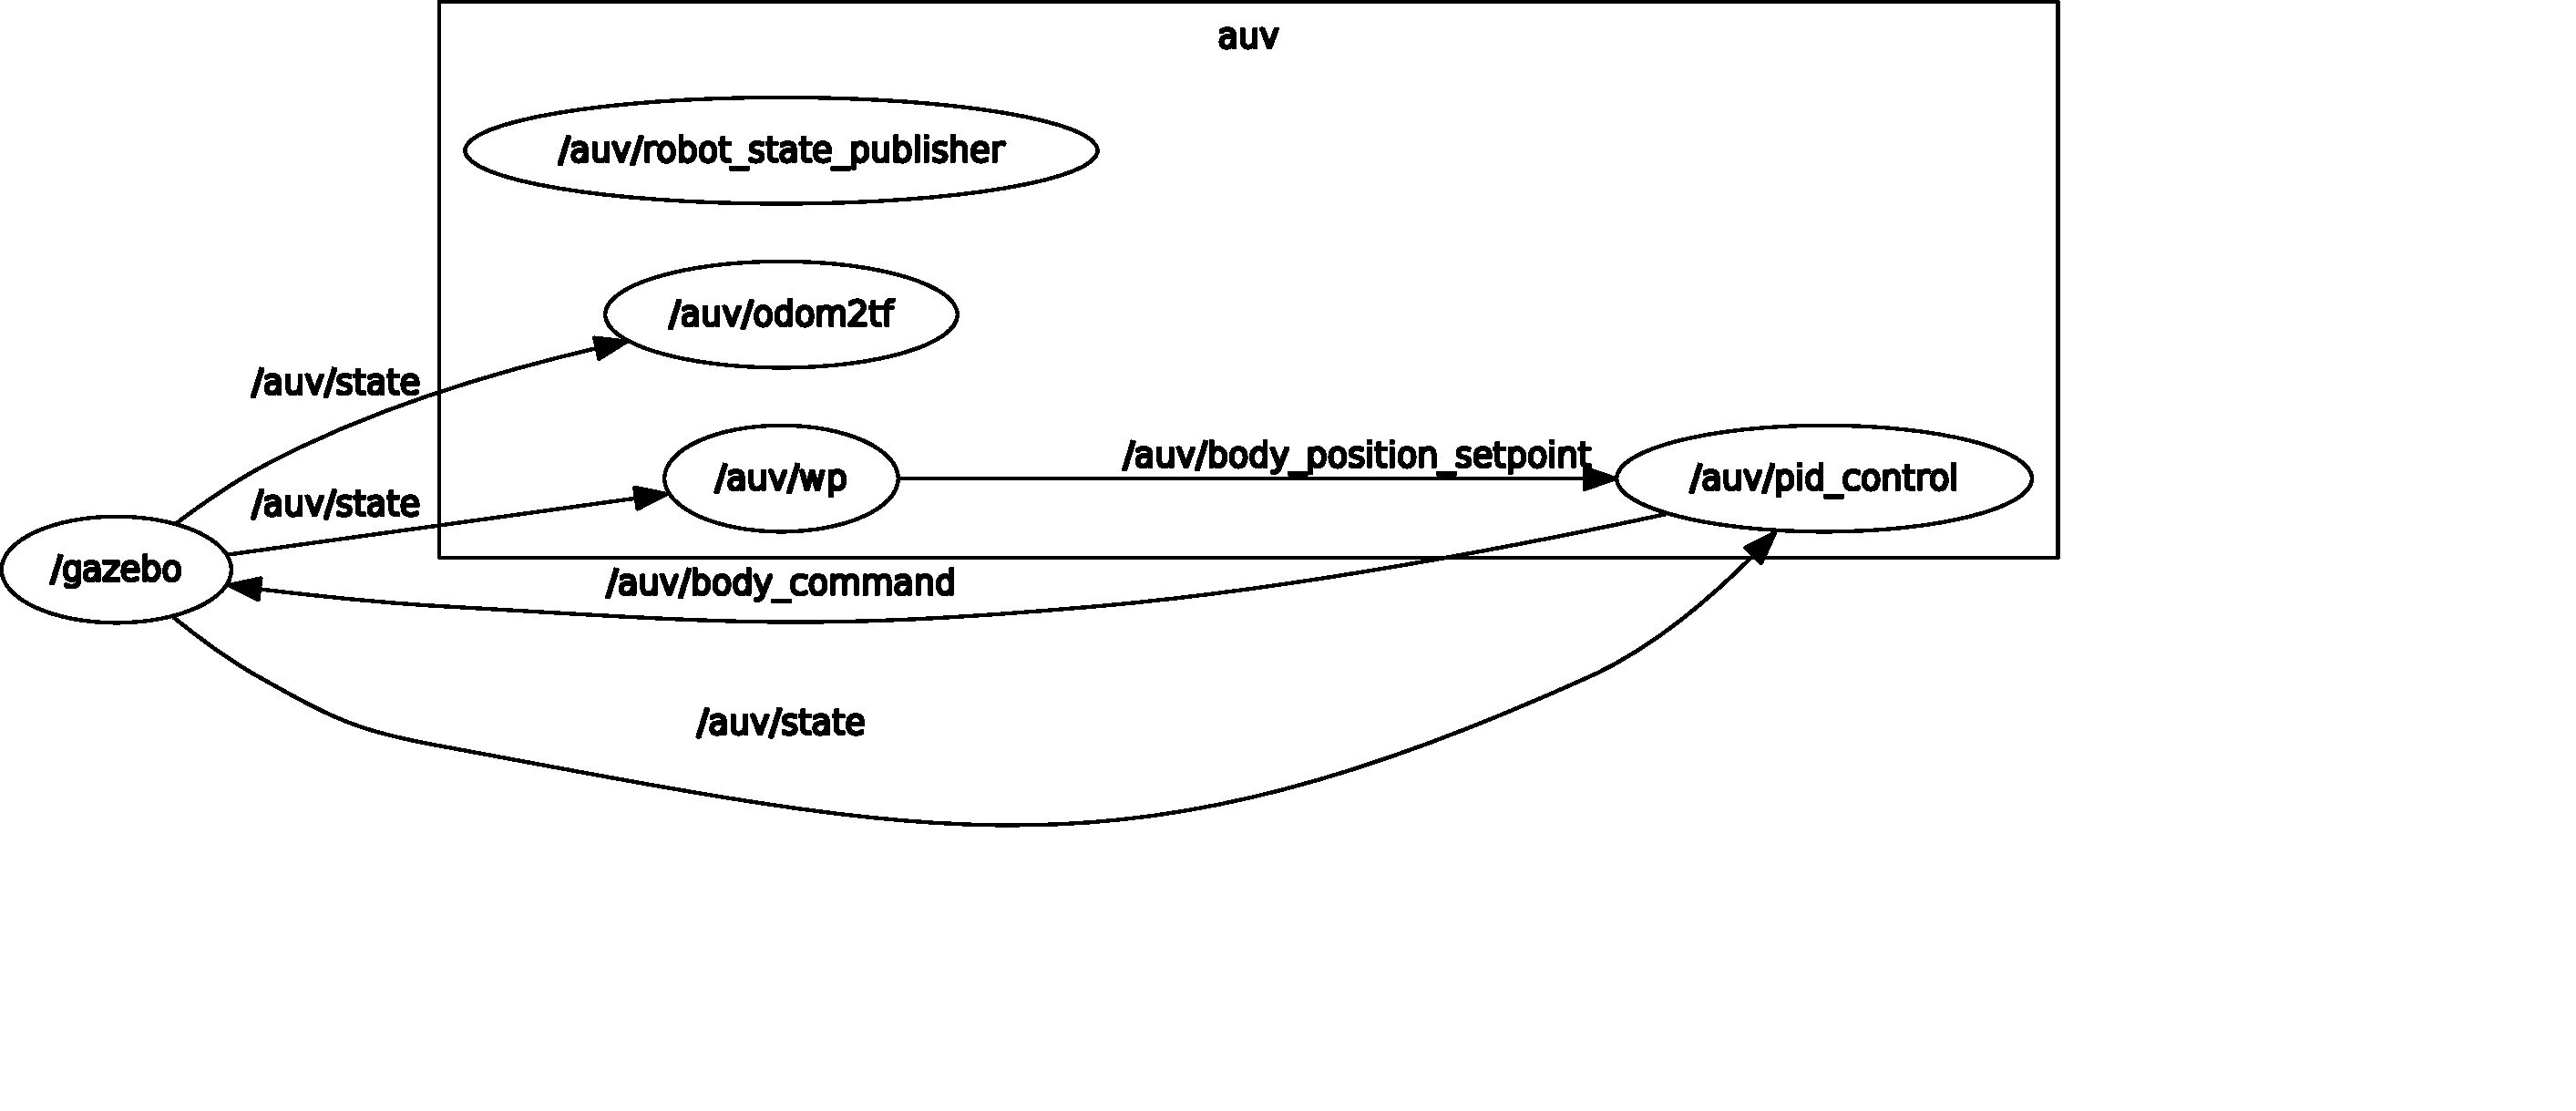
\includegraphics[width=.8\linewidth]{graph_wp}
\end{figure}

Two GUI are launched: 
\begin{itemize}
 \item UWsim is an underwater rendering software that displays the AUV in a realistic environment
 \item RViz is a visualizer and displays the current pose estimate (red) and the current waypoint to be followed (green)
\end{itemize}
The Gazebo dynamic simulator is also launched without GUI. In case of issues with UWsim display, the launch file can be used with Gazebo GUI instead of UWSim:
\begin{center}\defaultstyle
\begin{lstlisting}
roslaunch ecn_rasom auv.launch uwsim:=false
  \end{lstlisting}
  \end{center}

Manually defined setpoints can be easily published by using \texttt{rqt} message publisher, to check if the waypoints can be followed (maximum depth, etc.).\\

The goal is to modify the source and waypoint list in order to loop through the waypoints (go back to waypoint 0 after the last one was reached).
The structure of the \texttt{setpoint} message can be found with:
\begin{center}\defaultstyle
\begin{lstlisting}
rosmsg show geometry_msgs/PoseStamped
\end{lstlisting}
\end{center}
which gives:
\begin{center}\defaultstyle
\begin{lstlisting}
std_msgs/Header header
  uint32 seq
  time stamp
  string frame_id
geometry_msgs/Pose pose
  geometry_msgs/Point position
    float64 x
    float64 y
    float64 z
  geometry_msgs/Quaternion orientation
    float64 x
    float64 y
    float64 z
    float64 w
\end{lstlisting}
\end{center}
The header is already written but you have to define the pose section from the reading of the loaded waypoint file.
A function is available to write the $i-$th waypoint into the \texttt{setpoint} message:
\begin{center}\cppstyle
\begin{lstlisting}
writeWP(int idx);
\end{lstlisting}
\end{center}
Remember that the AUV may not reach perfectly the desired position, so you should cycle to the next waypoint when the position error is below a given threshold.
Two thresholds are loaded from the YAML file: \texttt{thr} and \texttt{thr\_angle}, that may be tuned accordingly to the desired accuracy.\\
The current position of the AUV can be found on the topic \texttt{/auv/state} and is of type \texttt{nav\_msgs/Odometry} with a structure similar to \texttt{geometry\_msgs/PoseStamped}, and where we are interested only
in the \texttt{pose} section.\\


%\section{Modification and tuning of the robot}
%
%The underwater robot itself is defined in the \texttt{auv.xacro} file. Check the available sensors and thrusters and find the available motions from the thruster map.
%You can add or modify the thrusters if needed. The thruster control matrix is computed automatically, however the gains of the PID are not tuned accordingly.

%\subsection{Basics of URDF}
%
%The \texttt{xacro} format allows using variables to generate the URDF model of a robot. 
%In this format, the robot is composed of links and joints. In our case we will assume that the AUV has only one link and no joints.
%
%In the example the AUV is composed of one cylinder, which is described under the \texttt{visual} tag.
%A tutorial is available at \texttt{http://wiki.ros.org/urdf/Tutorials/Building a Visual Robot Model with URDF from Scratch}
%
%In addition to the main body, thruster links can be defined with the \texttt{xacro:thruster\_link} tag, as  shown in the example.
%The xyz position and the roll-pitch-yaw orientation between the main body and the thruster has to be indicated.

%\section{Low-level tuning}
%
%The gains of the PID can be tuned online through Dynamic Reconfigure in (\texttt{rqt}).
%The Dynamic Reconfigure plugin can be used to change the PID gains without exiting the simulator.
%Once acceptable values have been found for the gains, you may update the \texttt{auv\_control.yaml} file to set the default values.

\section{Pose estimation from Extended Kalman Filter}

The architecture used until then is quite unrealistic.
Indeed, data on the topic \texttt{/auv/state} is the ground truth in terms of absolute position and velocity of the AUV (it is coming
directly from the simulator).
In this section we will replace it by an EKF estimator and see the problems that arise. The new graph will be:
\begin{figure}[h]\centering
 \includegraphics[width=\linewidth]{graph_ekf}
\end{figure}

Here, Gazebo is still publishing the ground truth but on the \texttt{/auv/ground\_truth} topic. This data is processed (noise is added) and republished from two simulated sensors:
\begin{enumerate}
  \item A depth sensor publishing a pose on \texttt{/auv/depth} where only the Z-position is meaningful
  \item A USBL device publishing a pose on \texttt{/auv/usbl} where only the X and Y positions and Z orientation (yaw) are meaningful
\end{enumerate}
Gazebo is also publishing simulated data from the IMU on the \texttt{/auv/imu\_data} topic. 
Finally, the Gazebo gui is not visible anymore (like an actual underwater vehicle) and RViz displays the estimate of the AUV (in red). 
For comparison purpose, the ground truth is displayed in blue. The setpoint is still displayed in green.

The three sensor data (depth, USBL and IMU) should be fused by the EKF node in order to output an estimate of the state on the \texttt{/auv/state} topic that is used by the PID and your waypoint node.

Two launch files have to be run to do so:
\begin{itemize}
 \item \texttt{roslaunch ecn\_rasom auv\_estim.launch} for all built-in nodes
 \item \texttt{roslaunch ecn\_rasom ekf.launch} for the EKF and your node
\end{itemize}

The \texttt{ekf.launch} should be modified in order to:
\begin{itemize}
 \item run your waypoint node
 \item use the EKF node with available sensors
\end{itemize}
Documentation of the EKF node can be found on the \link{http://docs.ros.org/lunar/api/robot_localization/html/index.html}{\texttt{robot\_localization} package website}.
This node creates a 15-components (6 pose, 6 velocities and 3 accelerations) state estimate.
The parameters of this node should be modified so that the EKF node
subscribes to the available data topics. The boolean tables should
also be updated in order to tell which components of the state are measured by each of the sensors. 

Do not hesitate to run the EKF with only a partial knowledge of the state (only IMU for instance) in order to see the effect on the localization accuracy.

\section{Back to mission control}



\end{document}
